% generated by gen_wave_col_fig.py -- do not edit by hand
\documentclass[10pt]{standalone}
\usepackage{helvet}
\renewcommand{\familydefault}{\sfdefault}
\usepackage{amsmath}
\usepackage{tikz}
\usetikzlibrary{patterns,arrows.meta}
\definecolor{csleep}{HTML}{D9D9D9}
\definecolor{cpark}{HTML}{F8CBAD}
\definecolor{cread}{HTML}{DDEBF7}
\definecolor{cwrite}{HTML}{FCE4D6}
\definecolor{cmiss}{HTML}{F4B6B6}
\definecolor{cjoin}{HTML}{FFE699}
\definecolor{cld}{HTML}{C6E0B4}
\definecolor{cfpu}{HTML}{FFE699}
\definecolor{ccall}{HTML}{C00000}
\newcommand{\fss}{\fontsize{5.6}{6.4}\selectfont}
\newcommand{\fv}{\fontsize{5.0}{5.6}\selectfont}
\newcommand{\fvs}{\fontsize{4.5}{5.0}\selectfont}
\begin{document}
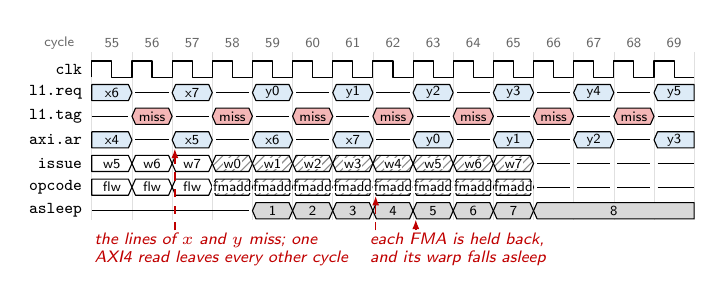
\begin{tikzpicture}[x=1cm, y=1cm,
  wire/.style={draw=black, line width=0.4pt, line join=round},
  gridline/.style={draw=black!12, line width=0.25pt},
  call/.style={draw=ccall, line width=0.5pt, dashed, -{Latex[length=1.2mm, width=0.9mm]}},
  callt/.style={font=\fss\itshape, text=ccall, inner sep=0.8pt, align=left}]

\node[font=\fv, text=black!60] at (1.305,-0.120) {55};
\node[font=\fv, text=black!60] at (1.815,-0.120) {56};
\node[font=\fv, text=black!60] at (2.325,-0.120) {57};
\node[font=\fv, text=black!60] at (2.835,-0.120) {58};
\node[font=\fv, text=black!60] at (3.345,-0.120) {59};
\node[font=\fv, text=black!60] at (3.855,-0.120) {60};
\node[font=\fv, text=black!60] at (4.365,-0.120) {61};
\node[font=\fv, text=black!60] at (4.875,-0.120) {62};
\node[font=\fv, text=black!60] at (5.385,-0.120) {63};
\node[font=\fv, text=black!60] at (5.895,-0.120) {64};
\node[font=\fv, text=black!60] at (6.405,-0.120) {65};
\node[font=\fv, text=black!60] at (6.915,-0.120) {66};
\node[font=\fv, text=black!60] at (7.425,-0.120) {67};
\node[font=\fv, text=black!60] at (7.935,-0.120) {68};
\node[font=\fv, text=black!60] at (8.445,-0.120) {69};
\draw[gridline] (1.050,-0.240) -- (1.050,-2.370);
\draw[gridline] (1.560,-0.240) -- (1.560,-2.370);
\draw[gridline] (2.070,-0.240) -- (2.070,-2.370);
\draw[gridline] (2.580,-0.240) -- (2.580,-2.370);
\draw[gridline] (3.090,-0.240) -- (3.090,-2.370);
\draw[gridline] (3.600,-0.240) -- (3.600,-2.370);
\draw[gridline] (4.110,-0.240) -- (4.110,-2.370);
\draw[gridline] (4.620,-0.240) -- (4.620,-2.370);
\draw[gridline] (5.130,-0.240) -- (5.130,-2.370);
\draw[gridline] (5.640,-0.240) -- (5.640,-2.370);
\draw[gridline] (6.150,-0.240) -- (6.150,-2.370);
\draw[gridline] (6.660,-0.240) -- (6.660,-2.370);
\draw[gridline] (7.170,-0.240) -- (7.170,-2.370);
\draw[gridline] (7.680,-0.240) -- (7.680,-2.370);
\draw[gridline] (8.190,-0.240) -- (8.190,-2.370);
\draw[gridline] (8.700,-0.240) -- (8.700,-2.370);
\node[anchor=east, font=\fv, text=black!60] at (0.950,-0.120) {cycle};
\node[anchor=east, font=\fss\ttfamily, inner sep=0.5pt] at (0.950,-0.450) {clk};
\draw[wire] (1.050,-0.552) -- (1.050,-0.348) -- (1.305,-0.348) -- (1.305,-0.552) -- (1.560,-0.552) -- (1.560,-0.348) -- (1.815,-0.348) -- (1.815,-0.552) -- (2.070,-0.552) -- (2.070,-0.348) -- (2.325,-0.348) -- (2.325,-0.552) -- (2.580,-0.552) -- (2.580,-0.348) -- (2.835,-0.348) -- (2.835,-0.552) -- (3.090,-0.552) -- (3.090,-0.348) -- (3.345,-0.348) -- (3.345,-0.552) -- (3.600,-0.552) -- (3.600,-0.348) -- (3.855,-0.348) -- (3.855,-0.552) -- (4.110,-0.552) -- (4.110,-0.348) -- (4.365,-0.348) -- (4.365,-0.552) -- (4.620,-0.552) -- (4.620,-0.348) -- (4.875,-0.348) -- (4.875,-0.552) -- (5.130,-0.552) -- (5.130,-0.348) -- (5.385,-0.348) -- (5.385,-0.552) -- (5.640,-0.552) -- (5.640,-0.348) -- (5.895,-0.348) -- (5.895,-0.552) -- (6.150,-0.552) -- (6.150,-0.348) -- (6.405,-0.348) -- (6.405,-0.552) -- (6.660,-0.552) -- (6.660,-0.348) -- (6.915,-0.348) -- (6.915,-0.552) -- (7.170,-0.552) -- (7.170,-0.348) -- (7.425,-0.348) -- (7.425,-0.552) -- (7.680,-0.552) -- (7.680,-0.348) -- (7.935,-0.348) -- (7.935,-0.552) -- (8.190,-0.552) -- (8.190,-0.348) -- (8.445,-0.348) -- (8.445,-0.552) -- (8.700,-0.552);
\node[anchor=east, font=\fss\ttfamily, inner sep=0.5pt] at (0.950,-0.750) {l1.req};
\draw[wire, fill=cread] (1.050,-0.647) -- (1.515,-0.647) -- (1.560,-0.750) -- (1.515,-0.852) -- (1.050,-0.852) -- (1.050,-0.750) -- cycle;
\node[font=\fv, inner sep=0pt] at (1.305,-0.750) {x6};
\draw[wire] (1.605,-0.750) -- (2.025,-0.750);
\draw[wire, fill=cread] (2.115,-0.647) -- (2.535,-0.647) -- (2.580,-0.750) -- (2.535,-0.852) -- (2.115,-0.852) -- (2.070,-0.750) -- cycle;
\node[font=\fv, inner sep=0pt] at (2.325,-0.750) {x7};
\draw[wire] (2.625,-0.750) -- (3.045,-0.750);
\draw[wire, fill=cread] (3.135,-0.647) -- (3.555,-0.647) -- (3.600,-0.750) -- (3.555,-0.852) -- (3.135,-0.852) -- (3.090,-0.750) -- cycle;
\node[font=\fv, inner sep=0pt] at (3.345,-0.750) {y0};
\draw[wire] (3.645,-0.750) -- (4.065,-0.750);
\draw[wire, fill=cread] (4.155,-0.647) -- (4.575,-0.647) -- (4.620,-0.750) -- (4.575,-0.852) -- (4.155,-0.852) -- (4.110,-0.750) -- cycle;
\node[font=\fv, inner sep=0pt] at (4.365,-0.750) {y1};
\draw[wire] (4.665,-0.750) -- (5.085,-0.750);
\draw[wire, fill=cread] (5.175,-0.647) -- (5.595,-0.647) -- (5.640,-0.750) -- (5.595,-0.852) -- (5.175,-0.852) -- (5.130,-0.750) -- cycle;
\node[font=\fv, inner sep=0pt] at (5.385,-0.750) {y2};
\draw[wire] (5.685,-0.750) -- (6.105,-0.750);
\draw[wire, fill=cread] (6.195,-0.647) -- (6.615,-0.647) -- (6.660,-0.750) -- (6.615,-0.852) -- (6.195,-0.852) -- (6.150,-0.750) -- cycle;
\node[font=\fv, inner sep=0pt] at (6.405,-0.750) {y3};
\draw[wire] (6.705,-0.750) -- (7.125,-0.750);
\draw[wire, fill=cread] (7.215,-0.647) -- (7.635,-0.647) -- (7.680,-0.750) -- (7.635,-0.852) -- (7.215,-0.852) -- (7.170,-0.750) -- cycle;
\node[font=\fv, inner sep=0pt] at (7.425,-0.750) {y4};
\draw[wire] (7.725,-0.750) -- (8.145,-0.750);
\draw[wire, fill=cread] (8.235,-0.647) -- (8.700,-0.647) -- (8.700,-0.750) -- (8.700,-0.852) -- (8.235,-0.852) -- (8.190,-0.750) -- cycle;
\node[font=\fv, inner sep=0pt] at (8.445,-0.750) {y5};
\node[anchor=east, font=\fss\ttfamily, inner sep=0.5pt] at (0.950,-1.050) {l1.tag};
\draw[wire] (1.050,-1.050) -- (1.515,-1.050);
\draw[wire, fill=cmiss] (1.605,-0.947) -- (2.025,-0.947) -- (2.070,-1.050) -- (2.025,-1.152) -- (1.605,-1.152) -- (1.560,-1.050) -- cycle;
\node[font=\fv, inner sep=0pt] at (1.815,-1.050) {miss};
\draw[wire] (2.115,-1.050) -- (2.535,-1.050);
\draw[wire, fill=cmiss] (2.625,-0.947) -- (3.045,-0.947) -- (3.090,-1.050) -- (3.045,-1.152) -- (2.625,-1.152) -- (2.580,-1.050) -- cycle;
\node[font=\fv, inner sep=0pt] at (2.835,-1.050) {miss};
\draw[wire] (3.135,-1.050) -- (3.555,-1.050);
\draw[wire, fill=cmiss] (3.645,-0.947) -- (4.065,-0.947) -- (4.110,-1.050) -- (4.065,-1.152) -- (3.645,-1.152) -- (3.600,-1.050) -- cycle;
\node[font=\fv, inner sep=0pt] at (3.855,-1.050) {miss};
\draw[wire] (4.155,-1.050) -- (4.575,-1.050);
\draw[wire, fill=cmiss] (4.665,-0.947) -- (5.085,-0.947) -- (5.130,-1.050) -- (5.085,-1.152) -- (4.665,-1.152) -- (4.620,-1.050) -- cycle;
\node[font=\fv, inner sep=0pt] at (4.875,-1.050) {miss};
\draw[wire] (5.175,-1.050) -- (5.595,-1.050);
\draw[wire, fill=cmiss] (5.685,-0.947) -- (6.105,-0.947) -- (6.150,-1.050) -- (6.105,-1.152) -- (5.685,-1.152) -- (5.640,-1.050) -- cycle;
\node[font=\fv, inner sep=0pt] at (5.895,-1.050) {miss};
\draw[wire] (6.195,-1.050) -- (6.615,-1.050);
\draw[wire, fill=cmiss] (6.705,-0.947) -- (7.125,-0.947) -- (7.170,-1.050) -- (7.125,-1.152) -- (6.705,-1.152) -- (6.660,-1.050) -- cycle;
\node[font=\fv, inner sep=0pt] at (6.915,-1.050) {miss};
\draw[wire] (7.215,-1.050) -- (7.635,-1.050);
\draw[wire, fill=cmiss] (7.725,-0.947) -- (8.145,-0.947) -- (8.190,-1.050) -- (8.145,-1.152) -- (7.725,-1.152) -- (7.680,-1.050) -- cycle;
\node[font=\fv, inner sep=0pt] at (7.935,-1.050) {miss};
\draw[wire] (8.235,-1.050) -- (8.700,-1.050);
\node[anchor=east, font=\fss\ttfamily, inner sep=0.5pt] at (0.950,-1.350) {axi.ar};
\draw[wire, fill=cread] (1.050,-1.247) -- (1.515,-1.247) -- (1.560,-1.350) -- (1.515,-1.452) -- (1.050,-1.452) -- (1.050,-1.350) -- cycle;
\node[font=\fv, inner sep=0pt] at (1.305,-1.350) {x4};
\draw[wire] (1.605,-1.350) -- (2.025,-1.350);
\draw[wire, fill=cread] (2.115,-1.247) -- (2.535,-1.247) -- (2.580,-1.350) -- (2.535,-1.452) -- (2.115,-1.452) -- (2.070,-1.350) -- cycle;
\node[font=\fv, inner sep=0pt] at (2.325,-1.350) {x5};
\draw[wire] (2.625,-1.350) -- (3.045,-1.350);
\draw[wire, fill=cread] (3.135,-1.247) -- (3.555,-1.247) -- (3.600,-1.350) -- (3.555,-1.452) -- (3.135,-1.452) -- (3.090,-1.350) -- cycle;
\node[font=\fv, inner sep=0pt] at (3.345,-1.350) {x6};
\draw[wire] (3.645,-1.350) -- (4.065,-1.350);
\draw[wire, fill=cread] (4.155,-1.247) -- (4.575,-1.247) -- (4.620,-1.350) -- (4.575,-1.452) -- (4.155,-1.452) -- (4.110,-1.350) -- cycle;
\node[font=\fv, inner sep=0pt] at (4.365,-1.350) {x7};
\draw[wire] (4.665,-1.350) -- (5.085,-1.350);
\draw[wire, fill=cread] (5.175,-1.247) -- (5.595,-1.247) -- (5.640,-1.350) -- (5.595,-1.452) -- (5.175,-1.452) -- (5.130,-1.350) -- cycle;
\node[font=\fv, inner sep=0pt] at (5.385,-1.350) {y0};
\draw[wire] (5.685,-1.350) -- (6.105,-1.350);
\draw[wire, fill=cread] (6.195,-1.247) -- (6.615,-1.247) -- (6.660,-1.350) -- (6.615,-1.452) -- (6.195,-1.452) -- (6.150,-1.350) -- cycle;
\node[font=\fv, inner sep=0pt] at (6.405,-1.350) {y1};
\draw[wire] (6.705,-1.350) -- (7.125,-1.350);
\draw[wire, fill=cread] (7.215,-1.247) -- (7.635,-1.247) -- (7.680,-1.350) -- (7.635,-1.452) -- (7.215,-1.452) -- (7.170,-1.350) -- cycle;
\node[font=\fv, inner sep=0pt] at (7.425,-1.350) {y2};
\draw[wire] (7.725,-1.350) -- (8.145,-1.350);
\draw[wire, fill=cread] (8.235,-1.247) -- (8.700,-1.247) -- (8.700,-1.350) -- (8.700,-1.452) -- (8.235,-1.452) -- (8.190,-1.350) -- cycle;
\node[font=\fv, inner sep=0pt] at (8.445,-1.350) {y3};
\node[anchor=east, font=\fss\ttfamily, inner sep=0.5pt] at (0.950,-1.650) {issue};
\draw[wire, fill=white] (1.050,-1.547) -- (1.515,-1.547) -- (1.560,-1.650) -- (1.515,-1.752) -- (1.050,-1.752) -- (1.050,-1.650) -- cycle;
\node[font=\fv, inner sep=0pt] at (1.305,-1.650) {w5};
\draw[wire, fill=white] (1.605,-1.547) -- (2.025,-1.547) -- (2.070,-1.650) -- (2.025,-1.752) -- (1.605,-1.752) -- (1.560,-1.650) -- cycle;
\node[font=\fv, inner sep=0pt] at (1.815,-1.650) {w6};
\draw[wire, fill=white] (2.115,-1.547) -- (2.535,-1.547) -- (2.580,-1.650) -- (2.535,-1.752) -- (2.115,-1.752) -- (2.070,-1.650) -- cycle;
\node[font=\fv, inner sep=0pt] at (2.325,-1.650) {w7};
\draw[wire, fill=white, pattern=north east lines, pattern color=black!45] (2.625,-1.547) -- (3.045,-1.547) -- (3.090,-1.650) -- (3.045,-1.752) -- (2.625,-1.752) -- (2.580,-1.650) -- cycle;
\node[font=\fv, fill=white, inner sep=0.25pt] at (2.835,-1.650) {w0};
\draw[wire, fill=white, pattern=north east lines, pattern color=black!45] (3.135,-1.547) -- (3.555,-1.547) -- (3.600,-1.650) -- (3.555,-1.752) -- (3.135,-1.752) -- (3.090,-1.650) -- cycle;
\node[font=\fv, fill=white, inner sep=0.25pt] at (3.345,-1.650) {w1};
\draw[wire, fill=white, pattern=north east lines, pattern color=black!45] (3.645,-1.547) -- (4.065,-1.547) -- (4.110,-1.650) -- (4.065,-1.752) -- (3.645,-1.752) -- (3.600,-1.650) -- cycle;
\node[font=\fv, fill=white, inner sep=0.25pt] at (3.855,-1.650) {w2};
\draw[wire, fill=white, pattern=north east lines, pattern color=black!45] (4.155,-1.547) -- (4.575,-1.547) -- (4.620,-1.650) -- (4.575,-1.752) -- (4.155,-1.752) -- (4.110,-1.650) -- cycle;
\node[font=\fv, fill=white, inner sep=0.25pt] at (4.365,-1.650) {w3};
\draw[wire, fill=white, pattern=north east lines, pattern color=black!45] (4.665,-1.547) -- (5.085,-1.547) -- (5.130,-1.650) -- (5.085,-1.752) -- (4.665,-1.752) -- (4.620,-1.650) -- cycle;
\node[font=\fv, fill=white, inner sep=0.25pt] at (4.875,-1.650) {w4};
\draw[wire, fill=white, pattern=north east lines, pattern color=black!45] (5.175,-1.547) -- (5.595,-1.547) -- (5.640,-1.650) -- (5.595,-1.752) -- (5.175,-1.752) -- (5.130,-1.650) -- cycle;
\node[font=\fv, fill=white, inner sep=0.25pt] at (5.385,-1.650) {w5};
\draw[wire, fill=white, pattern=north east lines, pattern color=black!45] (5.685,-1.547) -- (6.105,-1.547) -- (6.150,-1.650) -- (6.105,-1.752) -- (5.685,-1.752) -- (5.640,-1.650) -- cycle;
\node[font=\fv, fill=white, inner sep=0.25pt] at (5.895,-1.650) {w6};
\draw[wire, fill=white, pattern=north east lines, pattern color=black!45] (6.195,-1.547) -- (6.615,-1.547) -- (6.660,-1.650) -- (6.615,-1.752) -- (6.195,-1.752) -- (6.150,-1.650) -- cycle;
\node[font=\fv, fill=white, inner sep=0.25pt] at (6.405,-1.650) {w7};
\draw[wire] (6.705,-1.650) -- (7.125,-1.650);
\draw[wire] (7.215,-1.650) -- (7.635,-1.650);
\draw[wire] (7.725,-1.650) -- (8.145,-1.650);
\draw[wire] (8.235,-1.650) -- (8.700,-1.650);
\node[anchor=east, font=\fss\ttfamily, inner sep=0.5pt] at (0.950,-1.950) {opcode};
\draw[wire, fill=white] (1.050,-1.848) -- (1.515,-1.848) -- (1.560,-1.950) -- (1.515,-2.053) -- (1.050,-2.053) -- (1.050,-1.950) -- cycle;
\node[font=\fvs, inner sep=0pt] at (1.305,-1.950) {flw};
\draw[wire, fill=white] (1.605,-1.848) -- (2.025,-1.848) -- (2.070,-1.950) -- (2.025,-2.053) -- (1.605,-2.053) -- (1.560,-1.950) -- cycle;
\node[font=\fvs, inner sep=0pt] at (1.815,-1.950) {flw};
\draw[wire, fill=white] (2.115,-1.848) -- (2.535,-1.848) -- (2.580,-1.950) -- (2.535,-2.053) -- (2.115,-2.053) -- (2.070,-1.950) -- cycle;
\node[font=\fvs, inner sep=0pt] at (2.325,-1.950) {flw};
\draw[wire, fill=white, pattern=north east lines, pattern color=black!45] (2.625,-1.848) -- (3.045,-1.848) -- (3.090,-1.950) -- (3.045,-2.053) -- (2.625,-2.053) -- (2.580,-1.950) -- cycle;
\node[font=\fvs, fill=white, inner sep=0.25pt] at (2.835,-1.950) {fmadd};
\draw[wire, fill=white, pattern=north east lines, pattern color=black!45] (3.135,-1.848) -- (3.555,-1.848) -- (3.600,-1.950) -- (3.555,-2.053) -- (3.135,-2.053) -- (3.090,-1.950) -- cycle;
\node[font=\fvs, fill=white, inner sep=0.25pt] at (3.345,-1.950) {fmadd};
\draw[wire, fill=white, pattern=north east lines, pattern color=black!45] (3.645,-1.848) -- (4.065,-1.848) -- (4.110,-1.950) -- (4.065,-2.053) -- (3.645,-2.053) -- (3.600,-1.950) -- cycle;
\node[font=\fvs, fill=white, inner sep=0.25pt] at (3.855,-1.950) {fmadd};
\draw[wire, fill=white, pattern=north east lines, pattern color=black!45] (4.155,-1.848) -- (4.575,-1.848) -- (4.620,-1.950) -- (4.575,-2.053) -- (4.155,-2.053) -- (4.110,-1.950) -- cycle;
\node[font=\fvs, fill=white, inner sep=0.25pt] at (4.365,-1.950) {fmadd};
\draw[wire, fill=white, pattern=north east lines, pattern color=black!45] (4.665,-1.848) -- (5.085,-1.848) -- (5.130,-1.950) -- (5.085,-2.053) -- (4.665,-2.053) -- (4.620,-1.950) -- cycle;
\node[font=\fvs, fill=white, inner sep=0.25pt] at (4.875,-1.950) {fmadd};
\draw[wire, fill=white, pattern=north east lines, pattern color=black!45] (5.175,-1.848) -- (5.595,-1.848) -- (5.640,-1.950) -- (5.595,-2.053) -- (5.175,-2.053) -- (5.130,-1.950) -- cycle;
\node[font=\fvs, fill=white, inner sep=0.25pt] at (5.385,-1.950) {fmadd};
\draw[wire, fill=white, pattern=north east lines, pattern color=black!45] (5.685,-1.848) -- (6.105,-1.848) -- (6.150,-1.950) -- (6.105,-2.053) -- (5.685,-2.053) -- (5.640,-1.950) -- cycle;
\node[font=\fvs, fill=white, inner sep=0.25pt] at (5.895,-1.950) {fmadd};
\draw[wire, fill=white, pattern=north east lines, pattern color=black!45] (6.195,-1.848) -- (6.615,-1.848) -- (6.660,-1.950) -- (6.615,-2.053) -- (6.195,-2.053) -- (6.150,-1.950) -- cycle;
\node[font=\fvs, fill=white, inner sep=0.25pt] at (6.405,-1.950) {fmadd};
\draw[wire] (6.705,-1.950) -- (7.125,-1.950);
\draw[wire] (7.215,-1.950) -- (7.635,-1.950);
\draw[wire] (7.725,-1.950) -- (8.145,-1.950);
\draw[wire] (8.235,-1.950) -- (8.700,-1.950);
\node[anchor=east, font=\fss\ttfamily, inner sep=0.5pt] at (0.950,-2.250) {asleep};
\draw[wire] (1.050,-2.250) -- (3.045,-2.250);
\draw[wire, fill=csleep] (3.135,-2.147) -- (3.555,-2.147) -- (3.600,-2.250) -- (3.555,-2.353) -- (3.135,-2.353) -- (3.090,-2.250) -- cycle;
\node[font=\fv, inner sep=0pt] at (3.345,-2.250) {1};
\draw[wire, fill=csleep] (3.645,-2.147) -- (4.065,-2.147) -- (4.110,-2.250) -- (4.065,-2.353) -- (3.645,-2.353) -- (3.600,-2.250) -- cycle;
\node[font=\fv, inner sep=0pt] at (3.855,-2.250) {2};
\draw[wire, fill=csleep] (4.155,-2.147) -- (4.575,-2.147) -- (4.620,-2.250) -- (4.575,-2.353) -- (4.155,-2.353) -- (4.110,-2.250) -- cycle;
\node[font=\fv, inner sep=0pt] at (4.365,-2.250) {3};
\draw[wire, fill=csleep] (4.665,-2.147) -- (5.085,-2.147) -- (5.130,-2.250) -- (5.085,-2.353) -- (4.665,-2.353) -- (4.620,-2.250) -- cycle;
\node[font=\fv, inner sep=0pt] at (4.875,-2.250) {4};
\draw[wire, fill=csleep] (5.175,-2.147) -- (5.595,-2.147) -- (5.640,-2.250) -- (5.595,-2.353) -- (5.175,-2.353) -- (5.130,-2.250) -- cycle;
\node[font=\fv, inner sep=0pt] at (5.385,-2.250) {5};
\draw[wire, fill=csleep] (5.685,-2.147) -- (6.105,-2.147) -- (6.150,-2.250) -- (6.105,-2.353) -- (5.685,-2.353) -- (5.640,-2.250) -- cycle;
\node[font=\fv, inner sep=0pt] at (5.895,-2.250) {6};
\draw[wire, fill=csleep] (6.195,-2.147) -- (6.615,-2.147) -- (6.660,-2.250) -- (6.615,-2.353) -- (6.195,-2.353) -- (6.150,-2.250) -- cycle;
\node[font=\fv, inner sep=0pt] at (6.405,-2.250) {7};
\draw[wire, fill=csleep] (6.705,-2.147) -- (8.700,-2.147) -- (8.700,-2.250) -- (8.700,-2.353) -- (6.705,-2.353) -- (6.660,-2.250) -- cycle;
\node[font=\fv, inner sep=0pt] at (7.680,-2.250) {8};
\node[callt, anchor=north west] at (1.050,-2.500) {the lines of $x$ and $y$ miss; one\\AXI4 read leaves every other cycle};
\draw[call] (2.105,-2.500) -- (2.105,-1.462);
\node[callt, anchor=north west] at (4.550,-2.500) {each FMA is held back,\\and its warp falls asleep};
\draw[call] (4.655,-2.500) -- (4.655,-2.062);
\draw[call] (5.165,-2.500) -- (5.165,-2.362);
\end{tikzpicture}
\end{document}
